\documentclass{article}
\setlength{\parskip}{0pt} % esp. entre parrafos
\setlength{\parindent}{20pt} % esp. al inicio de un parrafo
\usepackage{amsmath} % mates
\usepackage{listings}
\usepackage{xcolor}
\usepackage[sort&compress,numbers]{natbib} % referencias
\usepackage{url} % que las URLs se vean lindos
\usepackage[top=10mm,left=20mm,right=20mm,bottom=25mm]{geometry} % \textbf{\textbf{}}margenes
\usepackage{hyperref} % ligas de URLs
\usepackage{graphicx} % poner figuras
\usepackage{caption}
\usepackage{subcaption}
\usepackage[spanish]{babel} % otros idiomas
\hypersetup{
    colorlinks=true,
    linkcolor=blue,
    filecolor=blue,      
    urlcolor=blue,
}
\renewcommand{\lstlistingname}{Código}
\definecolor{codeblack}{rgb}{0,0.6,0}
\definecolor{codegray}{rgb}{0.5,0.5,0.5}
\definecolor{codepurple}{rgb}{0.58,0,0.82}
\definecolor{backcolour}{rgb}{0.95,0.95,0.92}
\lstdefinestyle{mystyle}{
    backgroundcolor=\color{backcolour},   
    commentstyle=\color{codeblack},
    keywordstyle=\color{blue},
    numberstyle=\tiny\color{codegray},
    stringstyle=\color{codeblack},
    basicstyle=\ttfamily\footnotesize,
    breakatwhitespace=false,         
    breaklines=true,                 
    keepspaces=true,                 
    numbers=left,                    
    numbersep=5pt,                  
    showspaces=false,                
    showstringspaces=false,
    showtabs=false,                  
    tabsize=2
}
\lstset{style=mystyle}

\title{"P9" Interacciones entre partículas}
\author{NESTOR}
\date {Abril 2022}

\begin{document}

\maketitle

\section{Objetivo}\label{obj}
El objetivo de la práctica consiste en un modelo simplificado para los fenómenos de atracción y repulsión de física .Supongamos que contemos con $n$ partículas que habitan un cuadro unitario bidimensional y que cada partícula tiene una carga eléctrica, distribuida independientemente e normalmente al azar entre [$-1,1]$. Cargas de un mismo signo producirán una repulsión mientras cargas opuestas resultan en una atracción la magnitud de la fuerza estará proporcional a la diferencia de magnitud de las cargas (mayores diferencias resultando en fuerzas mayores), y además la fuerza será inversamente proporcional a la distancia euclideana entre las partículas \cite{elisa1}.

\section{Desarrollo}\label{des}
Basandome en el desarrollo en la \href{https://github.com/satuelisa/Simulation/blob/master/Particles/creation.py}{codificación} implementado por E. Schaeffer y todas las instrucciones se encuentran en el  \href{https://github.com/NestorZeus/SIMULACION-COMPUTACIONAL-DE-NANOMATERIALES/tree/main/P9}{repositorio} de N. Rodríguez en GitHub.\\

Para comenzar se hace primero generar la función para generar partículas de atracción y repulsión con esto para poder visualizar la masa

\begin{lstlisting} [caption=Generamos las partículas, label=codigo2, language=Python]
import numpy as np
import pandas as pd
from random import uniform 
import matplotlib.pyplot as plt
paso = 256 // 10
niveles = [i/256 for i in range(0, 256, paso)]
eps = 0.001
\end{lstlisting}

Generamos las posiciones de las partículas en "$x$ y $y$", se les asigna una carga y una masa con números random uniformemente con la finalidad de asignar masas variables.

\begin{lstlisting}[caption=Partículas en "$x$ y $y$", label=codigo2, language=Python]
if __name__ == "__main__":
    inicial=[]
    popen('rm -f p9p_t*.png') # borramos anteriores en el caso que lo hayamos corrido
    n = 25
    x = np.random.normal(size = n)
    y = np.random.normal(size = n)
    masa = [uniform(0,50)for i in range(n)]
    c = np.random.normal(size = n)
    #masa=[s * (-1) for s in masa]
\end{lstlisting}

Se realizó ya las masas variables, ahora se codifica que la masa cause un efecto ya que está asignada a una partícula, ya que con esto se hace varios pasos para que vayan avanzando las partículas, a continuación se muestra la codificación:
\begin{lstlisting}[caption=masa, label=codigo2, language=Python]
def fuerza(i, shared):
    p = shared.data
    n = shared.count
    pi = p.iloc[i]
    xi = pi.x
    yi = pi.y
    ci = pi.c
    mi = pi.masa
    fx, fy = 0, 0
    for k in range(n):
        pk = p.iloc[k]
        ck = pk.c
        mk = pk.masa
        dire_c = (-1)**(1 + (ci * ck < 0))
        dire_m = (-1)**(1 + (mi * mk > 0))
        factor_c = dire_c * fabs(ci - ck) / (sqrt(dx**2 + dy**2) + eps)
        factor_m = dire_m * fabs(mi - mk) / (sqrt(dx**2 + dy**2) + eps)
        fx -= dx * factor_m * factor_c
        fy -= dy * factor_m * factor_c
    return (fx, fy)
\end{lstlisting}

Generamos la correlación de rango de Spearman, esto nos ayudará a correlacionar las tres variables en una medida de asociación lineal que se utilizará para los rangos.

\begin{lstlisting}[caption=Spearman, label=codigo2, language=Python]
### Correlacion de rango de Spearman
    from scipy.stats import spearmanr
    stat, p = spearmanr(x, z)
    print("correlacion carga con velocidad")
    print('stat=%.3f, p=%.3f' % (stat, p))
    if p > 0.05:
        print('Probablemente dependiente')
    else:
        print('Probablemente independiente')
    print("correlacion masa con velocidad")
    stat2, p2 = spearmanr(y, z)
    print('stat=%.3f, p=%.3f' % (stat2, p2))
    if p2 > 0.05:
        print('Probablemente dependiente')
    else:
        print('Probablemente independiente')
\end{lstlisting}

\section{Resultados}\label{res}
\begin{table}[h!]
    \centering
    \caption{Correlacion de rango de Spearman para las partículas}
    \begin{tabular}{|r|r|r|r||r|r|r|r||r|r|r|r|}
    \hline
       Mediciónes & Estadística \\
       \hline\hline
        Relacion entre la velocidad con carga y velocidad con masa & $0.37567824$ porciento \\
        \hline
       Correlacion carga con velocidad  & stat=$0.380$, p=$0.061$ (Probablemente dependiente) \\
        \hline
       Correlacion masa con velocidad  & stat=$-0.285$, p=$0.167$ (Probablemente dependiente) \\
        \hline
    \end{tabular}
    \label{medir_R}
\end{table}

\begin{figure}
    \centering
    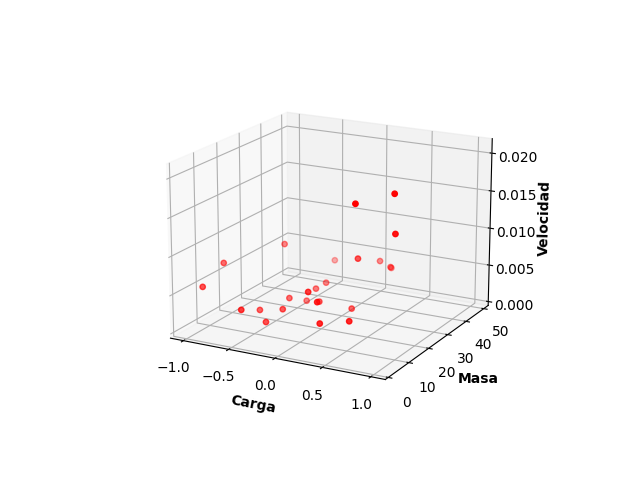
\includegraphics[width=200mm]{Figure_1.png}
    \caption{Partículas en la carga.}
    \label{figure}
\end{figure}
\begin{figure}
    \centering
    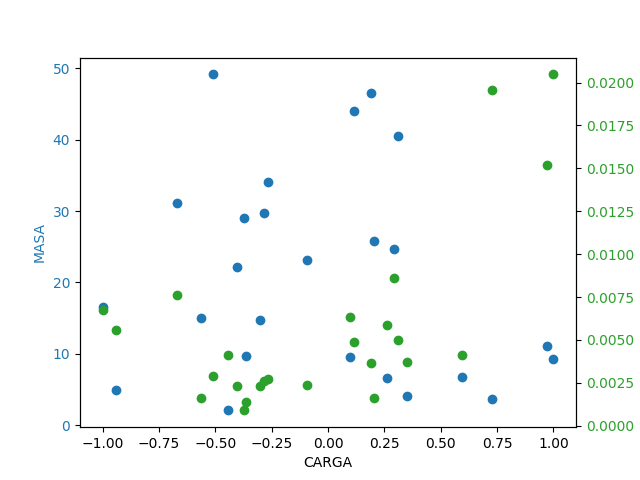
\includegraphics[width=180mm]{Figure_2.png}
    \caption{Comportamiento de carga.}
    \label{figure}
\end{figure}

\newpage
\section{Conclusiones}\label{}
Se concluye que las partículas se correlacionan con las tres variables con respecto a la carga y la menor velocidad ya que se encuentra la diferencia en velocidades.
\bibliographystyle{plainnat}
\bibliography{simulacion}
\end{document}
